\documentclass{article}
\usepackage[utf8]{inputenc}
\usepackage{geometry}
\usepackage{graphicx}
\usepackage{url,hyperref}
\usepackage{array}

\hypersetup{colorlinks,citecolor=red,urlcolor=blue} 
\newcolumntype{P}[1]{>{\raggedleft\arraybackslash}p{#1}}

\title{
	Web Information Extraction and Retrieval\\
	Programming Assignment 1: \\
	Crawler implementation
}

\author{
  Marko Prelevikj\\
  63130345\\
  \texttt{mp2638@student.uni-lj.si}
  \and
  Gojko Hajduković\\
  63180431\\
  \texttt{gh8590@student.uni-lj.si}
  \and
  Stefan Ivanišević\\
  63170405\\
  \texttt{si0539@student.uni-lj.si}
}
\date{April 2019}

\begin{document}

\maketitle

\section{Introduction}
With the size of the World Wide Web enlarging constantly and rapidly, web crawlers were made as emerging technology which became a key component of Web Search Engines, as well as many other businesses providing a help with crawling and extracting data from Web.Nowadays, there exist various crawler implementations developed for specific usage. In this paper we introduce our implementation of a stand-alone crawler which crawls \texttt{.gov.si} web pages and gathers all links, images and binary data. Implementation specifics and analysis of the obtained data are provided in the following sections.

\section{Implementation specifics}

The implementation of the web crawler is done in Scala, which is a functional programming language, offering a lot of syntactical sugars which make the development process easier.
We chose it in order to improve our programming skills in Scala, and also, learn a lot about its capabilities for concurrent programming.

\subsection{Dependencies}

To make the development process as easy as possible, we are using a number of dependencies. In this report, we are listing the once which are most significant, whilst the list of entire dependencies is available in the \texttt{build.sbt} file. 
\begin{itemize}
	\item \texttt{akka-actor} - providing us with the support of multi-threading through the concept of actor systems~\cite{Akka:ActorSystem}.
	\item \texttt{slick} - a functional relational mapping library to easily store data into the database~\cite{Slick}.
	\item \texttt{crawler-commons} - a library containing common utilities for crawlers~\cite{Crawler-commons}.
	\item \texttt{htmlunit} - headless browser which renders the html content of a provided URL~\cite{htmlunit}.
	\item \texttt{bigqueue} - a multithread-safe persistent queue for keeping the frontier~\cite{bigqueue}.
	\item \texttt{JSoup} - a library for HTML document parsing~\cite{jsoup}.
\end{itemize}

\subsection{Database modifications}

In order to make the implementation more insightful, we expanded the initial database with additional columns as follows:
\subsubsection{Table \texttt{page}}
We introduced the fields:
\begin{itemize}
    \item \texttt{hash} - SHA256 hash of the entire HTML content of the page, used for duplicate detection.
    \item \texttt{load\_time} - time needed to load the page by \texttt{HtmlUnit}
    \item \texttt{stored\_time} - when the page was added in the queue
\end{itemize}
\subsubsection{Table \texttt{page\_type}}
We introduced the following values:
\begin{itemize}
    \item \texttt{INVALID} - in case there has occurred an unknown error while loading the page
    \item \texttt{DISALLOWED} - if the page is not allowed by the \texttt{robots.txt} file
\end{itemize}

\subsubsection{Table \texttt{page\_data}}
We introduced the following column:
\begin{itemize}
    \item \texttt{filename} - canonical url of the stored file
\end{itemize}

\subsubsection{Storing process}

We altered the storing process as well. We omit a page entry of the type \textit{BINARY} which should be a reference to the \textit{image} or \textit{page\_data} table. Instead, we are linking the resources directly to the pages where they occurred. For example, if there had been an image linked to a page with \texttt{id = 1}, we enter an image entry with a reference to the page with \texttt{id = 1}.

\section{Crawler implementation}

The development process of the crawler was done in multiple iterations. In the first iteration, we developed all the required utilities to build the crawler upon. These utilities include: URL-canonicalization, \texttt{SiteMap} parsing, \texttt{robots.txt} parsing, database service to store the obtained data. Furthermore, we developed the core concepts, and the basic pipeline of how the crawler should interact with the frontier and the database. Finally, we created workers which are going to perform the crawling.

There are two versions of the crawler workers. First, we tried a naive implementation in~\ref{subsec:jitter} with jittered time between the requests to the same domain, which didn't turn out well. Next, we developed a more advanced version of the worker in~\ref{subsec:bf}, which implements a distributed breadth-first approach.

\subsection{Core concepts}

The following steps describe the process of fetching and storing the data retrieved from a given URL. Whenever we refer to processing of a page, we are referring to the following steps:
\begin{enumerate}
	\item frontier dequeueing - get the next page from the frontier
	\item \texttt{robots.txt} check - check whether the page is allowed in the \texttt{robots.txt}, skip it if not. If the \texttt{robots.txt} is missing - allow it by default
	\item page rendering - get the page content and HTTP status code using \texttt{HtmlUnit}
	\item data extraction - extract all the detected links pages and binary data in the page using \texttt{JSoup}
	\item data deduplication - detect the entries which already exist, and link them accordingly. 
	\item data storage - The duplicate detection is performed on a database level: if the URL exists - it is a duplicate, if it does not, it checks whether its hash code already exists, if it does not it is finally written into the database.
	\item frontier enqueueing - All the non-duplicate links, images, and binary data is enqueued in the frontier to be processed when they come in line.
	\item delay - after all the processing has been performed, the worker waits for at least \texttt{5s} until the next page is processed, depending on the presence of \texttt{robots.txt}.
	\item repeat the process for the rest of the entries
\end{enumerate}

Data dedpuplication is done in two steps. Firstly, if there exists an exact match for the provided url it is marked as a duplicate. Secondly, if there is an exact match of the \texttt{SHA256} hash of the HTML content of the page, it is marked as a duplicate. Both of these operations are performed on a database level, to increase the performance of the rest of the code.

\subsection{Version 1 - Jittered Delay} \label{subsec:jitter}

Our naive approach is consisted of having multiple workers, which are reading from the frontier and processing the upcoming page. Each of the workers are spawned with a $5s$ jittered delay, where the jittering is in the range from $2$ to $20$ seconds.

We introduced the jitter in order to reduce the probability of having the crawler processing a page from the same domain. Unfortunately, since the crawler is working in a breadth-first manner, it is highly unlikely to have two sequential pages from two different domains.

Since we are limited to a single host machine, which has a single IP address, it would mean that we need to synchronise all threads and have a semaphore which will determine the delay between the requests.

The low level of concurrency would effectively mean that the multi-threading is not as effective as it could be if the concurrency was independent among the threads. We support this fact by the fact that we obtained only $3500$ pages in $12h$ without downloading . Which lead us to the better approach, described in the section below. We illustrated our approach is illustrated in Figure~\ref{fig:1}.

\subsection{Version 2 - Distributed Breadth-First} \label{subsec:bf}

\begin{figure}
	\begin{minipage}{0.45\textwidth}
		\centering
		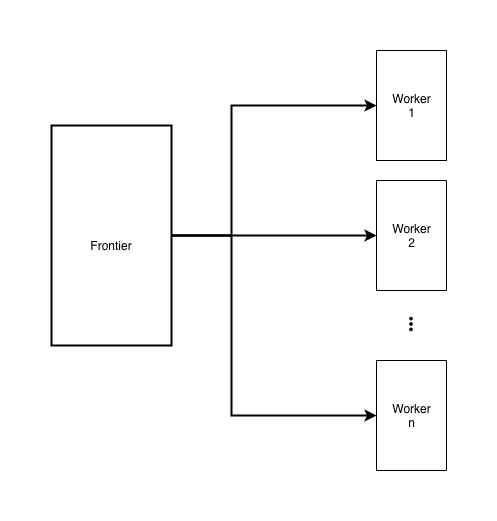
\includegraphics[width=0.9\textwidth]{jittered-delay.png}
		\caption{v.1.0 of the worker with a simultaneous access to the global frontier.}
		\label{fig:1}
	\end{minipage}\hfill
	\begin{minipage}{0.45\textwidth}
		\centering
		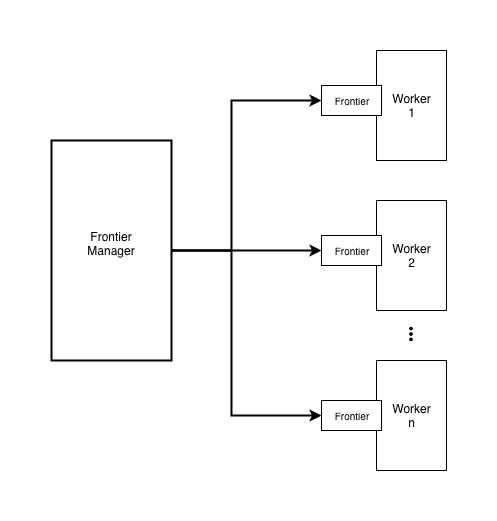
\includegraphics[width=0.9\textwidth]{frontier-manager.png}
		\caption{v2.0 of the worker with a \textit{Frontier Manager} which delegates the workload.}
		\label{fig:2}
	\end{minipage}
\end{figure}

To take full advantage of the concurrency we decided to distribute the frontier among the pool of workers. The distribution is done such that each worker is in charge of a single domain - a \textit{Domain Worker}, with the assumption that each of the domains has its own server. We illustrate this approach in Figure~\ref{fig:2}.

To achieve the distribution, we introduced a special kind of worker which we call a \textit{Frontier Manager}. Its purpose is to orchestrate the \textit{domain workers} and route the workload to each of the workers. 

By orchestration, we mean that the \textit{Frontier Manager} has the permission to spawn new workers, if there are more domains available than workers currently. Another very important task it has is to pick a new domain for the worker which has finished processing a given domain. This is a crucial task, as it keeps all of the resources at full capacity and therefore it can maximize the number of pages it processes in a given time period. Picking a new domain for a worker is performed randomly: when the request arrives, the manager extracts all non-processed domains and picks one at random. This is a reason why we have a really big wait time in the queue. We discuss this at more length in Section~\ref{sec:analysis}.

Additionally, the \textit{Frontier Manager} reroutes all the obtained links to the correct worker's frontier to be processed. If the given domain is currently inactive, then it keeps the pages in memory until it is chosen to be processed, when forwards them to the worker, and it resets the local state.

The \textit{Domain Worker} is checking its status every $15s$ and if the local frontier is empty, it sends a signal to the \textit{Frontier Manager} to get a new domain to process next. The delayed time between subsequent requests to the targetted server is not wasted by the worker, as it uses that time to enqueue all the incoming links from the \textit{Frontier Manager}, and to check its own status (this is implemented as a message to the standard output), and to act accordingly.


\section{Data Analysis}\label{sec:analysis}

After we have finished the development of our approach, we did two separate experiments. The first experiment was performed with the initial seed which we were provided. The second experiment was performed by extending the initial seed with 5 additional entries, which were picked at random from the site list obtained from the first experiment:
\begin{itemize}
	\item \url{http://www.evode.gov.si/},
	\item \url{http://www.fu.gov.si/},
	\item \url{http://www.mo.gov.si/},
	\item \url{http://www.arso.gov.si/},
	\item \url{http://www.mirs.gov.si/}
\end{itemize}

We illustrate the general statistics in Table~\ref{tab:1}. The number of pages in Table~\ref{tab:1} refers to the number of crawled pages of \texttt{HTML} data type and correspondingly, its detected duplicates. This discrepancy is due to easier implementation of the crawler. Thus, the overall number of pages is the sum of all pages, images, and page data, denoted with sum pages, at the bottom of the table. Our initial constraint was $100000$ pages, and we thought pages of type \texttt{HTML}, so our goal was to populate the database with at most $100000$ \texttt{HTML} pages. We also note that the binary data in the second experiment presents a much larger set because we scraped all binary data from the initial (extended) seed.

From the data, we can conclude that most of the sites are reusing their images throughout their pages, which is why we have a very high number of image duplicates. In the first experiment we have $\approx68\%$ image duplicates, and in the second case we have staggering $\approx83\%$ of duplicates. Whereas the number of duplicate pages detected by our duplicate detection technique (a simple \texttt{SHA256} hash of the HTML content) is quite small $\approx2.5\%$ in the first case, and $\approx3\%$ in the second. These findings are also expected, given the context of crawling \texttt{.gov.si} websites, which is a government web space and is supposed to be as informative as possible.

What we found curious is that we found a high percentage of invalid pages: first experiment $\approx12.0\%$, and in the second $\approx13.5\%$. A more detailed distribution of the \texttt{HTTP} status codes is shown in Table~\ref{tab:2}. It also shows us that there are quite a lot of broken links, with status $404$. Additionally, it reveals that our implementation of the URL canonicalization could be improved, since there is quite a big number of pages with status code $400$.

Additionally, since we expanded the \texttt{page} table of the database with the \texttt{load\_time} and \texttt{stored\_time} we were able to extract some additional statistics about our crawler. With  \texttt{load\_time} we were able to extract the distribution of the time required by \texttt{HtmlUnit} to render the provided URL. The visualization is shown in Figure~\ref{fig:3}. It can be noticed that the maximum time required to render the page is $\approx30s$, which is our upper limit for timing out the page and continuing with the next one.

Another metric which we were able to extract from our data \textit{queue wait time}. We obtained this statistic by modifying the \texttt{stored\_time} column to store the time when the entry has been enqueued in the frontier. To obtain the final metric, we simply subtract the \texttt{accessed\_time} and \texttt{stored\_time}. We present the visualization of the distribution of the \textit{queue wait time} metric in Figure~\ref{fig:4}. The average queue wait time in the first experiment is $111.057min$, whereas in the second it is $119.629min$. Some of the outliers shown in Figure~\ref{fig:4} indicate that the wait time has been more than $600min$. The reason why we have such a big wait time in some cases is due to the randomness we introduced on how the next site to be crawled is chosen and it indicates that it has been a wrong decision and it somewhat violates the \textit{breadth-first} paradigm of our crawler. In spite of this, relying on the fact that we keep the frontier order for each site we do achieve true \textit{distributed breadth-first} crawler. This was also indicated by following the trace of the program, which repeatedly showed us that the pages from the same domain are indeed processed in the same order. And this, of course, depends on the initial seed pages.


\begin{table}[hbt!]
	\centering
	\begin{tabular}{P{0.15\linewidth}|c|c}
		& Original seed & Extended seed \\ \hline
		running time [min] & 618 & 686  \\ \hline
		avg wait time [min] & 111.057 & 119.629 \\ \hline
		avg load time [ms] & 1351.347 & 1759.769 \\ \hline
		sites      & 288 & 327 \\ \hline
		pages      & 38268 & 58060 \\ \hline
		invalid pages & 4599 & 7847 \\ \hline
		disallowed pages & 214 & 541 \\ \hline
		duplicates & 971 & 1766 \\ \hline
		links & 1585648 & 2569510 \\ \hline
		images     & 94368 & 187924 \\ \hline
		avg images  per page  & 6.3567 & 8.520 \\ \hline
		duplicate images & 64638 & 155277 \\ \hline
		page data       & 28721 & 44761 \\ \hline
		avg page data per page    & 4.9853 & 6.170 \\ \hline
		duplicate data &11688 & 12593\\ \hline
		doc & 32 & 226 \\ \hline
		docx & 2 & 132 \\ \hline
		pdf & 230 & 941 \\ \hline
		sum pages* & 161357 & 290745 \\
	\end{tabular}
	\caption{General statistics of the experiments. *Sum pages is the sum of all pages, images and page data}
	\label{tab:1}
\end{table}

\begin{table}[hbt!]
	\centering
	\begin{tabular}{r|c|c}
		& Original seed & Extended seed \\ \hline
		400 & 1590 & 4043 \\ \hline
		401 & 10 & 14  \\ \hline
		403 & 22 & 46 \\ \hline
		404 & 2899 & 3692 \\ \hline
		410 & 14 & 12 \\ \hline
		500 & 25 & 15 \\ \hline
		501 & 1 & 0 \\ \hline
		502 & 20 & 0 \\ \hline
		503 & 14 & 21 \\
	\end{tabular}
	\caption{Status codes of the invalid pages. }
	\label{tab:2}
\end{table}


\begin{figure}
	\begin{minipage}{0.45\textwidth}
		\centering
		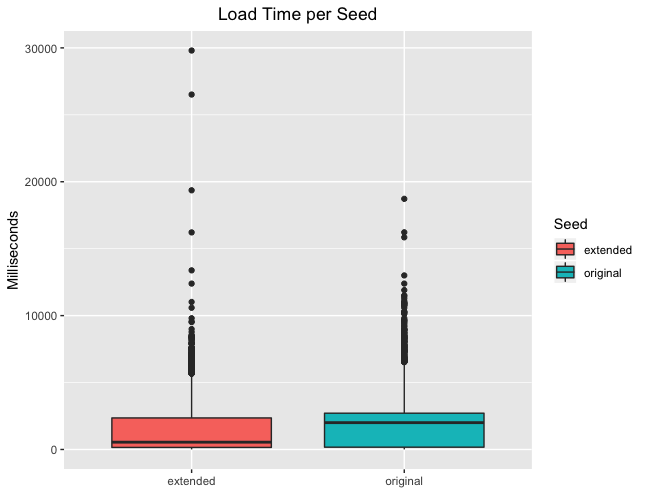
\includegraphics[width=0.9\textwidth]{load_time.png}
		\caption{Load time.}
		\label{fig:3}
	\end{minipage}\hfill
	\begin{minipage}{0.45\textwidth}
		\centering
		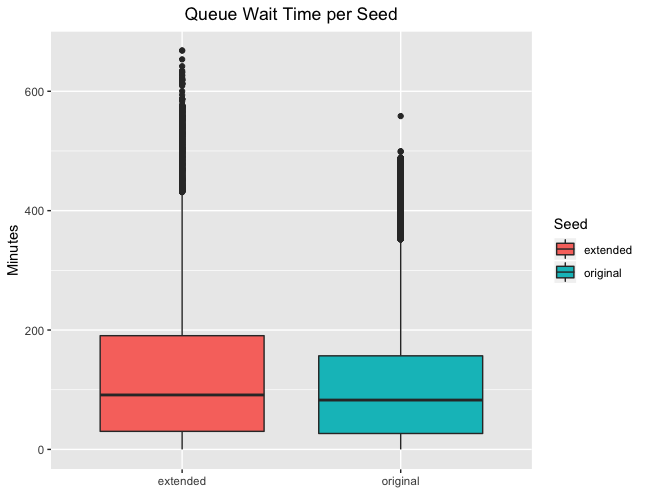
\includegraphics[width=0.9\textwidth]{queue_wait_time.png}
		\caption{Queue wait time.}
		\label{fig:4}
	\end{minipage}
\end{figure}

\subsection{Graph visualization}

Finally, we present how the pages are connected among each other on Figure~\ref{fig:5}. To present the connectivity graph we exploited the \texttt{link} table which we populated in our database. Since we have built a really big database, we were only able to visualize the part of the database which we are submitting along with this report. To visualize the graph, we used \href{https://gephi.org}{Gephi}, with the \textit{Fruchterman Reingold} layout method.

The graph is consisted of $723$ nodes and $13181$ links between them. The network's average degree is $18.231$, and its diameter is $121$. On Figure~\ref{fig:5} is also presented that there are $3$ main connected components. The colour of the node indicates its clustering coefficient, and the lighter the colour it is, the higher the coefficient is (pink indicates the highest clustering coefficient). According to \textit{PageRank}, the highest ranked page is \url{https://evem.gov.si/evem/cert/uporabnik/prijava.evem/}. 

\begin{figure}
	\centering
	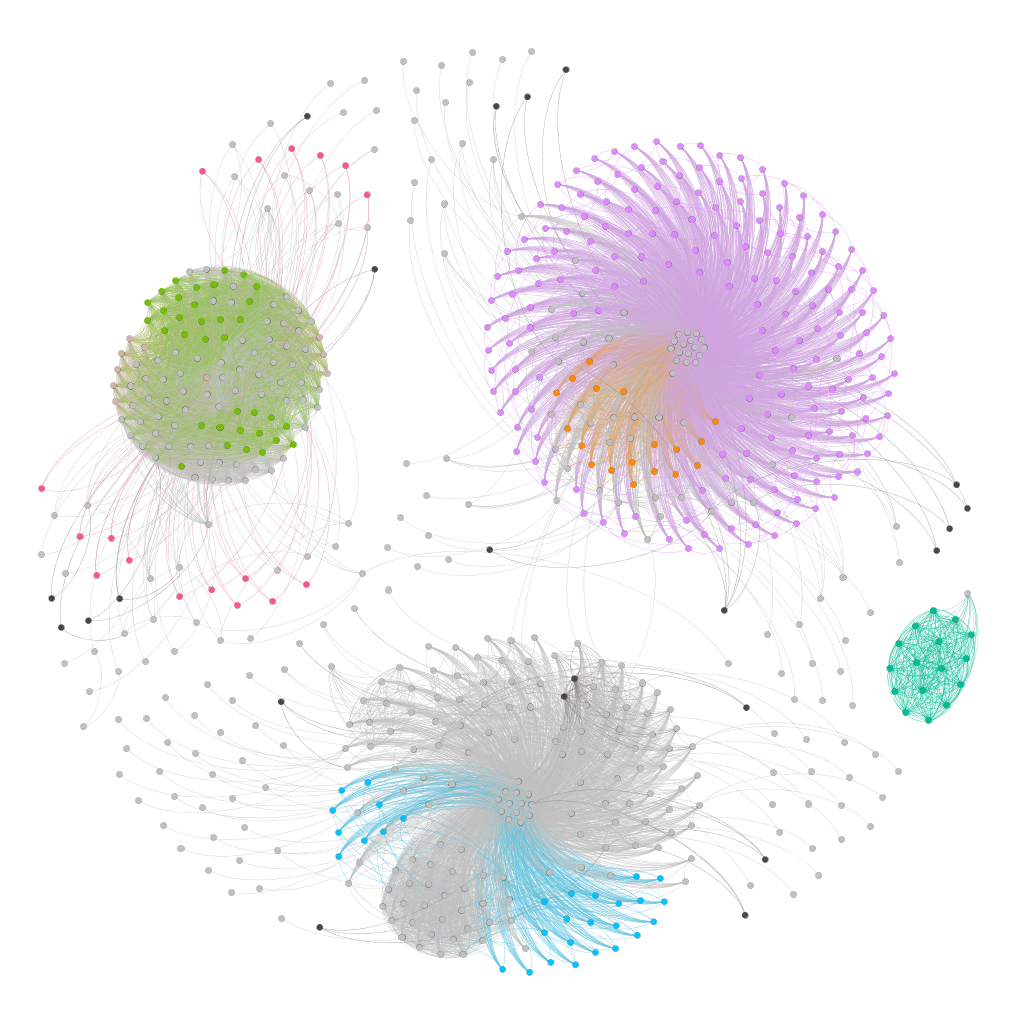
\includegraphics[width=0.6\textwidth]{reduced_graph.png}
	\caption{Graph visualization.}
	\label{fig:5}
\end{figure}

\section{Conclusion}
We introduced an efficient stand-alone web crawler which crawls selected web domains.In order to make crawler more efficient in the version v2.0 we introduced a architecture with a \textit{Frontier Manager} which distributes the frontier to a pool of workers, taking advantage of concurrency ultimately improving crawlers efficiency. Comparing our results with a professional software for crawling, Apache Nutch it crawls $\approx3.5$ times more pages than for selected initial seed and with HTML Unit it crawls  $\approx36$ times more pages.

\bibliographystyle{IEEEtran}
\bibliography{refs}

\end{document}
